\begin{figure}
\vspace{-0.4 cm}
\setlength{\abovecaptionskip}{0.3 cm}   
\setlength{\belowcaptionskip}{-0.4 cm}   
	\centering
    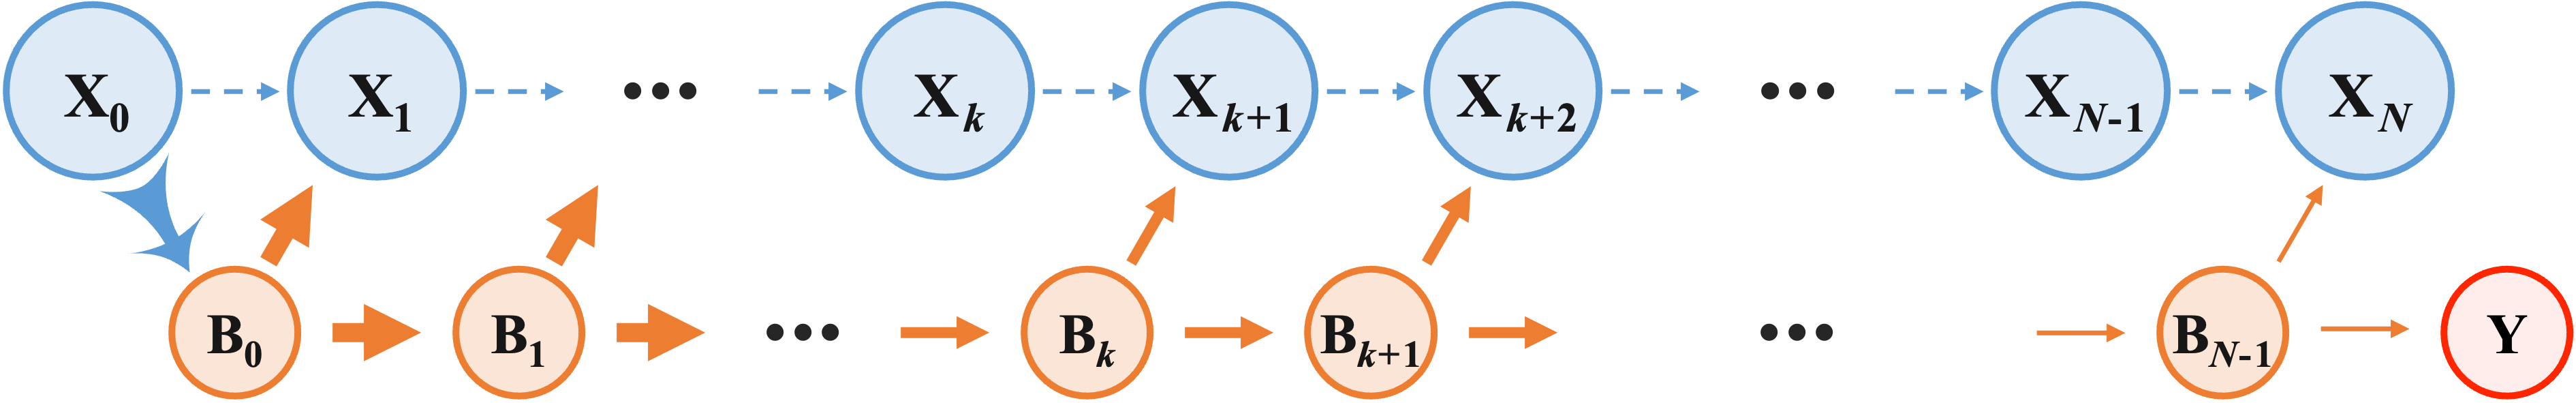
\includegraphics[width=\linewidth]{Figures/states.png}
    \caption{$N$ latent states are constructed for extracting and transferring the most relevant information of a set of $N+1$ modal states. The modal states are represented by $X_0$, $X_1$, ..., $X_{N-1}$, and $X_N$. This order is determined by the richness of the amount of information contained in the modalities. The latent states $B_0$, $B_1$, ..., $B_{N-1}$ represent the pathway for transferring the relevant information among $X$. Through the hierarchical structure, the most relevant information from $X_0$ to $X_N$ is gradually retained and distilled.}
    \label{fig:statesk}
\end{figure}